%
% 31-nullstellenc.tex -- Nullstellen von Polynomen über C
%
% (c) 2026 Prof Dr Andreas Müller
%
\subsection{Nullstellen von Polynomen über $\mathbb{C}$}
Hat man eine Nullstelle $\alpha$ eines Polynoms $p(X)\in K[X]$ gefunden,
die noch nicht im Koeffizientenkörper enthalten ist, kann man das Polynom
durch $X-\alpha$ dividieren.
Dabei entsteht ein neues Polynom $q(X) = p(X)/(X-\alpha)$,
aber die Koeffizienten dieses neuen Polynoms sind im Allgemeinen nicht
mehr in $K$, sondern in $K(\alpha)$.

\begin{beispiel}
Das Polynom $p(X)=X^2-2\in \mathbb{Q}[X]$ hat die Nullstelle
$\alpha_0=\sqrt[3]{2}$.
Division durch $X-\alpha_0=X-\sqrt[3]{2}$ ergibt ein Polynom vom Grad 2:
\[
\def\p{\phantom{)}}
\def\r{\raisebox{4pt}{\mathstrut}}
\def\m{\llap{$-$}}
\renewcommand{\arraycolsep}{2pt}
\begin{array}{rcrcrcrcrcrcrcrcrcr}
  (X^3 & &                     & &                   &-&             2) &:& (X &-& \!\sqrt[3]{2}) &=& X^2 &+& \!\sqrt[3]{2}X &+& \!\sqrt[3]{4}.\\
\m(X^3 &-&   \!\sqrt[3]{2}X^2) & &                   & &                & &    & &                & &     & &                & &               \\
\cline{1-3}
       & &   \!\sqrt[3]{2}X^2\p& &                   & &                & &    & &                & &     & &                & & \r            \\
       & &\m(\!\sqrt[3]{2}X^2\p&-&   \!\sqrt[3]{4}X) & &                & &    & &                & &     & &                & &               \\
\cline{3-5}
       & &                     & &   \!\sqrt[3]{4}X\p&-&             2\p& &    & &                & &     & &                & & \r            \\
       & &                     & &\m(\!\sqrt[3]{4}X\p&-& \!\sqrt[3]{8}) & &    & &                & &     & &                & &               \\
\cline{5-7}
       & &                     & &                   & &             0\p& &    & &                & &     & &                & & \r            \\
\end{array}
\]
Die weiteren Nullstellen von $X^3-2$ können als Lösungen der quadratischen Gleichung
\[
X^2 + \!\sqrt[3]{2} X + \!\sqrt[3]{4}=0
\]
gefunden werden, deren Koeffizienten nicht in $\mathbb{Q}$, aber in
$\mathbb{Q}(\!\sqrt[3]{2})$ liegen.
Die Lösungsformel liefert
\[
\alpha_\pm
=
-
\frac{\!\sqrt[3]{2}}2 \pm \!\sqrt{
\frac{\!\sqrt[3]{4}}{4} - \!\sqrt[3]{4}
}
=
-
\frac{\!\sqrt[3]{2}}2 \pm
\frac{\!\sqrt[3]{2}}{2}
\!\sqrt{-3}
=
\!\sqrt[3]{2}
\frac{-1\pm i\!\sqrt{3}}2.
\]
Beginnt man jedoch mit der Nullstelle $\alpha_+= \sqrt[3]{2}(-1+\!\sqrt{3})/2$,
dann ist das Quotientenpolynom
\[
(X^3-2) : (X-\alpha_+)
=
X^2
+
\!\sqrt[3]{2}\frac{-1+i\!\sqrt{3}}{2} X
+
\!\sqrt[3]{4}\frac{-1-i\!\sqrt{3}}2.
\]
Dieses Polynom hat die Nullstellen $\alpha_0$ und $\alpha_-$,
die Koeffizienten sind aber nicht in $\mathbb{Q}$, sondern in
$\mathbb{Q}((-1+i\!\sqrt{3})/2)\subset(\mathbb{Q}(\!\sqrt[3]{2},i)$.
\end{beispiel}

\begin{satz}[Fundamentalsatz der Algebra]
Ein Polynom $p(X)\in \mathbb{C}[X]$ hat alle Nullstellen in $\mathbb{C}$.
\end{satz}

%
% fig-fundamental.tex
%
% (c) 2026 Prof Dr Andreas Müller
%
\begin{figure}
\centering
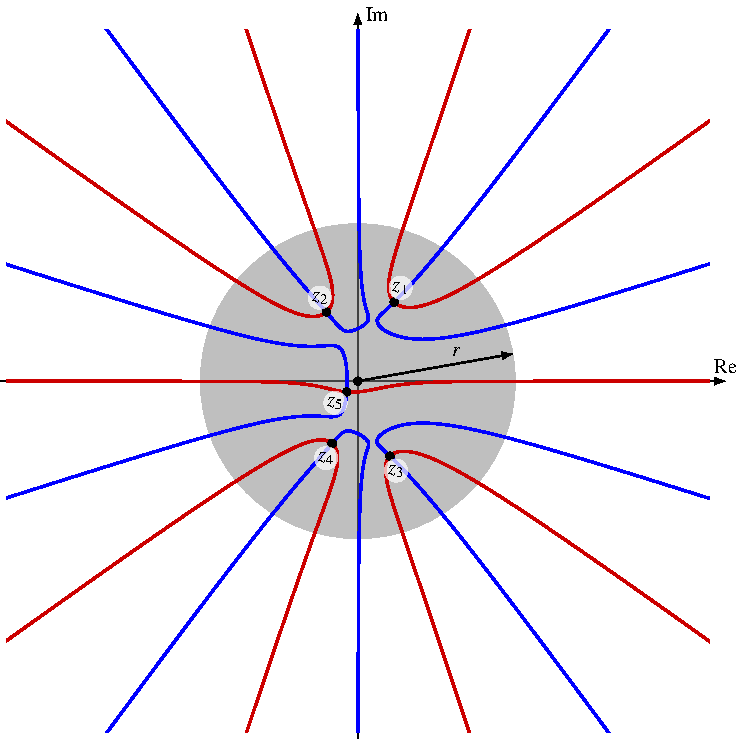
\includegraphics{chapters/010-komplex/images/fundamental.pdf}
\caption{Illustration von Gauss' Idee zum Beweis des Fundamentalsatzes
der Algebra anhand eines Polynoms $p(z)$ vom Grad 5.
Die roten Linien bestehen aus den Punkten $z$, für die der
Imaginärteil $\operatorname{Im} p(z)$ verschwindet.
Auf den blauen Kurven verschwindet der Realteil $\operatorname{Re}p(z)$.
Es kann höchstens 5 rote und blaue Kurven geben.
Ein grosser Kreis um den Nullpunkt schneidet abwechslungsweise rote und
blaue Kurven insgesamt je 10 mal.
Also müssen sich diese Kurven im Inneren des grauen Kreises schneiden.
Die Schnittpunkte sind Nullstellen $z_k$ des Polynoms
\label{buch:komplex:fig:fundamental}}
\end{figure}
%

Dieser Satz wird oft Carl Friedrich Gauss zugeschrieben.
\index{Gauss, Carl Friedrich}%
Sein erster Beweis ging von der folgenden Idee aus.
Sei $p(z)\in \mathbb{C}[z]$ ein normiertes Polynom vom Grad $n$.
Da eine Polynomgleichung höchstens $n$ Lösungen haben kann,
bestehen
\[
I=\{z\in\mathbb{C} \mid p(z) \in \mathbb{R} \}
\qquad\text{und}\qquad
R=\{z\in\mathbb{C} \mid p(z) \in i\mathbb{R} \}
\]
aus höchstens $n$ Kurven (Abbildung~\ref{buch:komplex:fig:fundamental},
blaue Kurven für $I$ und rote Kurven für $R$).
Ausserhalb eines grossen Kreises ist die führende Potenz $z^n$ dominant.
Auf dem Kreis mit Radius $r$ finden wir die Werte
\[
r^n (\cos n\varphi + i \sin n\varphi) + o(r^n),
\]
wobei abwechselnd der Real- bzw.~der Imaginärteil verschwinden.
Der Kreis schneidet also abwechseln eine Kurve von $R$ bzw.~von $I$
je $2n$ mal.
Da es sich jeweils nur um $n$ Kurven handelt, muss es im Inneren des
Kreises Schnittpunkte $z_k$ geben.
In einem Schnittpunkt einer roten und blauen Kurve sind sowohl 
Real- wie auch Imaginärteil $0$, er ist eine Nullstelle.

Die Beweisidee von Gauss hat jedoch eine Lücke: sie appelliert an 
intuitiv einleuchtende topologische Eigenschaften der komplexen
Ebene.
Dass solche Eigenschaften trotz ihrer Anschaulichkeit
nicht unbedingt selbstverständlich sind und einen Beweis erfordern,
wird auch in Kapitel~\ref{chapter:jordan} erläutert.

Der erste korrekte Beweis des Fundamentalsatzes wurde von 1814 von
Jean-Robert Argand publiziert \cite{buch:argand}.
\index{Argand, Jean-Robert}%
Argand war ein Buchhändler und Amateurmathematiker aus Genf,
wo er 1768 geboren wurde.
Er starb 1822 in Paris.
Sein Beweis des Fundamentalsatzes wird in Cauchys \emph{Cours d'analyse}
\index{Cauchy, Augustin-Louis}%
\cite{buch:cauchy} verwendet, der Autor Argand aber nicht erwähnt.

Wir werden den Fundamentalsatz in
Abschnitt~\ref{buch:analytisch:ganz:subsection:fundamentalsatz}
mit analytischen Hilfsmitteln beweisen.
Für die Analysis bedeutet dieser Satz, dass man mit dem Körper
$\mathbb{C}$ den Körper erreicht hat, indem jede Faktorisierungsaufgabe
von Polynome immer gelöst werden kann.
Dies hat zum Beispiel zur Konsquenz, dass sich das Integral
\index{Integral}%
jeder rationalen Funktion mit komplexen Koeffizienten immer
in geschlossener Form lösen lässt, wie
in Abschnitt~\ref{buch:ratint:section:bernoulli} gezeigt wird.
Das bedeutet aber noch nicht, dass das Integrationsproblem damit
gelöst ist, denn das Finden der Nullstellen ist immer noch ein
offenes Problem, welches im Kapitel~\ref{chapter:ratint} im Detail
untersucht wird.

